%%
%% StreamRing: A Cascading Architecture for Real-Time Detection of Blockchain Fraud Rings
%% Target: FinDS '26 Workshop (co-located with ACM SIGMOD 2026)
%%

%TC:macro \cite [option:text,text]
%TC:macro \citep [option:text,text]
%TC:macro \citet [option:text,text]
%TC:envir table 0 1
%TC:envir table* 0 1
%TC:envir tabular [ignore] word
%TC:envir displaymath 0 word
%TC:envir math 0 word
%TC:envir comment 0 0

\documentclass[sigconf, anonymous, review]{acmart}

\AtBeginDocument{%
  \providecommand\BibTeX{{%
    Bib\TeX}}}

\setcopyright{acmlicensed}
\copyrightyear{2026}
\acmYear{2026}
\acmConference[FinDS '26]{Workshop on Data Management for Modern Financial Systems}{May 31, 2026}{Bengaluru, India}

\usepackage{booktabs}
\usepackage{multirow}
\usepackage{graphicx}
\usepackage{xcolor}
\usepackage{algorithm}
\usepackage{algorithmic}
\usepackage{pifont}
\newcommand{\cmark}{\ding{51}}

\begin{document}

\title{StreamRing: A Cascading Architecture for Real-Time Detection of Blockchain Fraud Rings}

\author{Ahmad Zulfan}
\affiliation{%
  \institution{Bandung Institute of Technology}
  \city{Jakarta}
  \country{Indonesia}}
\email{ahmadzulfan352@gmail.com}

\author{Ahmad Jibril Hemdi}
\affiliation{%
 \institution{University of Copenhagen}
 \city{Copenhagen}
 \country{Denmark}}
\email{tbf947@alumni.ku.dk}

\author{Kyle Nathan Yahya}
\affiliation{%
  \institution{Technical University of Denmark}
  \city{Copenhagen}
  \country{Denmark}}
\email{s252786@dtu.dk}

\renewcommand{\shortauthors}{Zulfan et al.}

\begin{abstract}
Detecting coordinated fraud rings in blockchain transaction streams requires both structural pattern recognition and low-latency processing capabilities that no existing system provides simultaneously. Current GNN-based fraud detectors operate in batch mode on static snapshots, while streaming subgraph matching systems lack learned representations. We present \textsc{StreamRing}, a three-tier cascading architecture that unifies real-time subgraph pattern matching with graph neural network inference for fraud ring detection on Ethereum Classic. Tier~1 deploys an Incremental Fraud-Aware Subgraph Index (IFASI) with XGBoost, filtering 82\% of transactions in under 5\,ms. Tier~2 applies a temporal GNN for node-level escalation. Tier~3 performs subgraph-level fraud ring classification using a three-channel SubGNN encoder with contrastive regularization. Evaluated on 11.6M transactions spanning the DAO hack and 51\% attacks, StreamRing achieves 97.4\% precision at streaming throughput with all tiers meeting latency targets. Our novel Ring Detection Timeliness (RDT) metric shows 99.2\% of fraud ring members are detected before ring completion. We further demonstrate that feature masking is the only viable contrastive augmentation for fraud graphs---edge dropout degrades AUC by 4.1\% by destroying discriminative structural motifs.
\end{abstract}

\begin{CCSXML}
<ccs2012>
   <concept>
       <concept_id>10002951.10003317.10003347.10003356</concept_id>
       <concept_desc>Information systems~Stream management</concept_desc>
       <concept_significance>500</concept_significance>
   </concept>
   <concept>
       <concept_id>10010147.10010257.10010293.10010294</concept_id>
       <concept_desc>Computing methodologies~Neural networks</concept_desc>
       <concept_significance>300</concept_significance>
   </concept>
   <concept>
       <concept_id>10002978.10003029.10003031</concept_id>
       <concept_desc>Security and privacy~Economics of security and privacy</concept_desc>
       <concept_significance>300</concept_significance>
   </concept>
</ccs2012>
\end{CCSXML}

\ccsdesc[500]{Information systems~Stream management}
\ccsdesc[300]{Computing methodologies~Neural networks}
\ccsdesc[300]{Security and privacy~Economics of security and privacy}

\keywords{real-time fraud detection, subgraph matching, graph neural networks, streaming graphs, blockchain, fraud rings}

\received{25 March 2026}

\maketitle

%% ============================================================
\section{Introduction}
\label{sec:intro}

Cryptocurrency fraud exceeded an estimated \$17 billion in 2025~\cite{chainalysis2025}, with sophisticated fraud rings---coordinated groups of addresses executing phishing, money laundering, and double-spend attacks---posing the greatest threat to ecosystem trust. Unlike isolated fraudulent transactions, fraud rings manifest as \emph{subgraph patterns}: cycles indicating circular money flows, fan-out structures for fund splitting, and peeling chains for layering~\cite{spade2024}. Detecting these patterns in real time, before the ring completes its operation and funds become irrecoverable, remains an open challenge.

Two research communities have advanced toward this goal without converging. The \emph{continuous subgraph matching} community has developed algorithms such as TC-Match~\cite{tcmatch2024} and RapidFlow~\cite{rapidflow2022} that enumerate time-constrained pattern instances in streaming graphs with 10--100$\times$ speedups. The \emph{graph neural network} community has produced increasingly accurate fraud classifiers---ChronoWave-GNN~\cite{chronowave2025}, Elliptic++~\cite{ellipticpp2023}---but all operate in batch mode on static snapshots and classify individual transactions rather than coordinated rings. No existing system combines real-time subgraph matching with GNN-based fraud detection for streaming blockchain data.

We present \textsc{StreamRing}, a three-tier cascading architecture that bridges this gap. Each transaction is processed through progressively deeper analysis, with explicit latency budgets:
%
\begin{itemize}
    \item \textbf{Tier~1 ($<$5\,ms):} An Incremental Fraud-Aware Subgraph Index (IFASI) enumerates 12 structural patterns around each new edge and feeds counts to XGBoost.
    \item \textbf{Tier~2 ($<$50\,ms):} Escalated transactions undergo temporal GNN node scoring via SAGEConv with incremental graph updates.
    \item \textbf{Tier~3 ($<$500\,ms):} High-risk edges trigger subgraph extraction and fraud ring classification via a three-channel SubGNN encoder with contrastive regularization.
\end{itemize}

We evaluate \textsc{StreamRing} on Ethereum Classic data~\cite{ethereum_classic_kaggle}---11.6M transactions and 51.2M traces spanning the DAO hack and two 51\% attacks. Our contributions are:

\begin{enumerate}
    \item \textbf{StreamRing}, the first system unifying streaming subgraph matching with cascading GNN inference for real-time fraud ring detection, with all tiers meeting production latency constraints.
    \item \textbf{IFASI}, an incremental index with 12 fraud-specific pattern templates and temporal sliding windows, achieving sub-millisecond enumeration.
    \item The finding that \textbf{edge dropout destroys fraud discriminative patterns}, establishing feature masking as the principled augmentation for fraud graphs.
    \item \textbf{Ring Detection Timeliness (RDT)}, a metric measuring the fraction of ring members detected before ring completion, computed from actual model predictions on 166 fraud rings.
\end{enumerate}

%% ============================================================
\section{Related Work}
\label{sec:related}

\textbf{GNN-based blockchain fraud detection.} Weber et al.~\cite{weber2019} introduced the Elliptic dataset for Bitcoin AML with GCN baselines. Elmougy and Liu~\cite{ellipticpp2023} extended this to Elliptic++ with 822K addresses and four graph types. Lin et al.~\cite{chronowave2025} combined wavelet decomposition with temporal encoding (ChronoWave-GNN). P\'{e}rez-Cano and Jurado~\cite{perezcano2025} validated heterogeneous graph transformers. Asiri and Somasundaram~\cite{asiri2025} demonstrated GCN's advantage over traditional ML. All these methods operate in batch mode and perform node-level rather than ring-level classification.

\textbf{Temporal and streaming GNNs.} TGN~\cite{tgn2020} introduced per-node memory modules for event-level processing. EvolveGCN~\cite{evolvegcn2020} evolves GCN weights via GRU across snapshots. InkStream~\cite{inkstream2023} achieves 2.5--427$\times$ speedup via incremental inference, while RIPPLE++~\cite{ripple2025} scales to 20M+ updates. Shami and Kalavri~\cite{shami2025} identified challenges bridging GNN inference with Apache Flink streaming. None have been applied to fraud ring detection.

\textbf{Continuous subgraph matching.} TC-Match~\cite{tcmatch2024} introduced time-constrained CSM with a CSS index achieving 10--100$\times$ speedup over RapidFlow~\cite{rapidflow2022} and SymBi~\cite{symbi2021}. TurboFlux~\cite{turboflux2018} pioneered data-centric structures for streaming matching. These systems handle structural pattern enumeration but lack learned representations for classification.

\textbf{Subgraph-level fraud detection.} Spade+~\cite{spade2024} performs incremental dense subgraph peeling, deployed at Grab for fraud community detection. The Graph Feature Preprocessor~\cite{ibmgfp2024} demonstrated that explicit subgraph pattern counts outperform standalone GNNs by 20\%+ F1. Bit-CHetG~\cite{bitchetg2024} applied contrastive learning to Bitcoin laundering subgraphs. SubGNN~\cite{subgnn2020} proposed a three-channel encoder for general subgraph classification. StreamRing builds on SubGNN while adding streaming capabilities and fraud-specific pattern matching.

%% ============================================================
\section{Problem Formulation}
\label{sec:problem}

\textbf{Streaming transaction graph.} We model the blockchain as a temporal directed graph $\mathcal{G}_t = (\mathcal{V}_t, \mathcal{E}_t)$ evolving as new edges arrive. Each edge $e = (u, v, \tau, \mathbf{x}_e)$ carries attributes $\mathbf{x}_e$ (value, gas). Nodes $v \in \mathcal{V}_t$ have features $\mathbf{x}_v$ (degree, value statistics).

\textbf{Fraud ring.} A fraud ring $R = (\mathcal{V}_R, \mathcal{E}_R)$ is a connected subgraph where members coordinate fraudulent transactions within a temporal window. Its completion time is $\tau^*_R = \max_{e \in \mathcal{E}_R} \tau_e$.

\textbf{Detection problem.} Given streaming graph $\mathcal{G}_t$ and latency budget $\Delta$, for each new edge $e_t$, determine within $\Delta$ milliseconds whether $e_t$ belongs to a fraud ring and identify the ring members.

\textbf{Ring Detection Timeliness.} For ring $R$ with members $\mathcal{V}_R$ and completion $\tau^*_R$, let $\mathcal{D}_R$ be members detected before $\tau^*_R$:
\begin{equation}
    \text{RDT}(R) = |\mathcal{D}_R| / |\mathcal{V}_R|
\end{equation}
The aggregate $\overline{\text{RDT}} = \sum_R |\mathcal{D}_R| / \sum_R |\mathcal{V}_R|$ provides a member-weighted average.

%% ============================================================
\section{StreamRing Architecture}
\label{sec:arch}
Figure~\ref{fig:architecture} illustrates the three-tier cascading design of StreamRing. Each incoming edge is first processed by Tier~1, which uses the IFASI and an XGBoost classifier to filter safe transactions within 5~ms. Suspicious edges (those with a score above threshold) are escalated to Tier~2, where a temporal GNN scores nodes in an incrementally updated graph (50~ms budget). Edges that remain high-risk after node scoring proceed to Tier~3, which extracts a 2-hop temporal subgraph around the edge and performs final fraud ring classification using a SubGNN encoder with contrastive regularization (500~ms budget). This cascade ensures that only a small fraction of edges incur the full cost of subgraph-level analysis, enabling real-time throughput.

\textbf{Escalation thresholds.}
Tier\,1 escalates an edge when its XGBoost score exceeds a threshold~$\tau_{1}$
selected using Youden's~$J$ statistic on the warm-up period.
Tier\,2 escalates a node when its temporal-GNN logit exceeds~$\tau_{2}$,
similarly chosen via $J$-optimization on the validation split.
Both thresholds are fixed for all streaming periods and tuned only once during system warm-up.
This makes the cascade deterministic and ensures that only $\sim\!18\%$ of edges reach Tier\,3.

\begin{figure}[t]
    \centering
    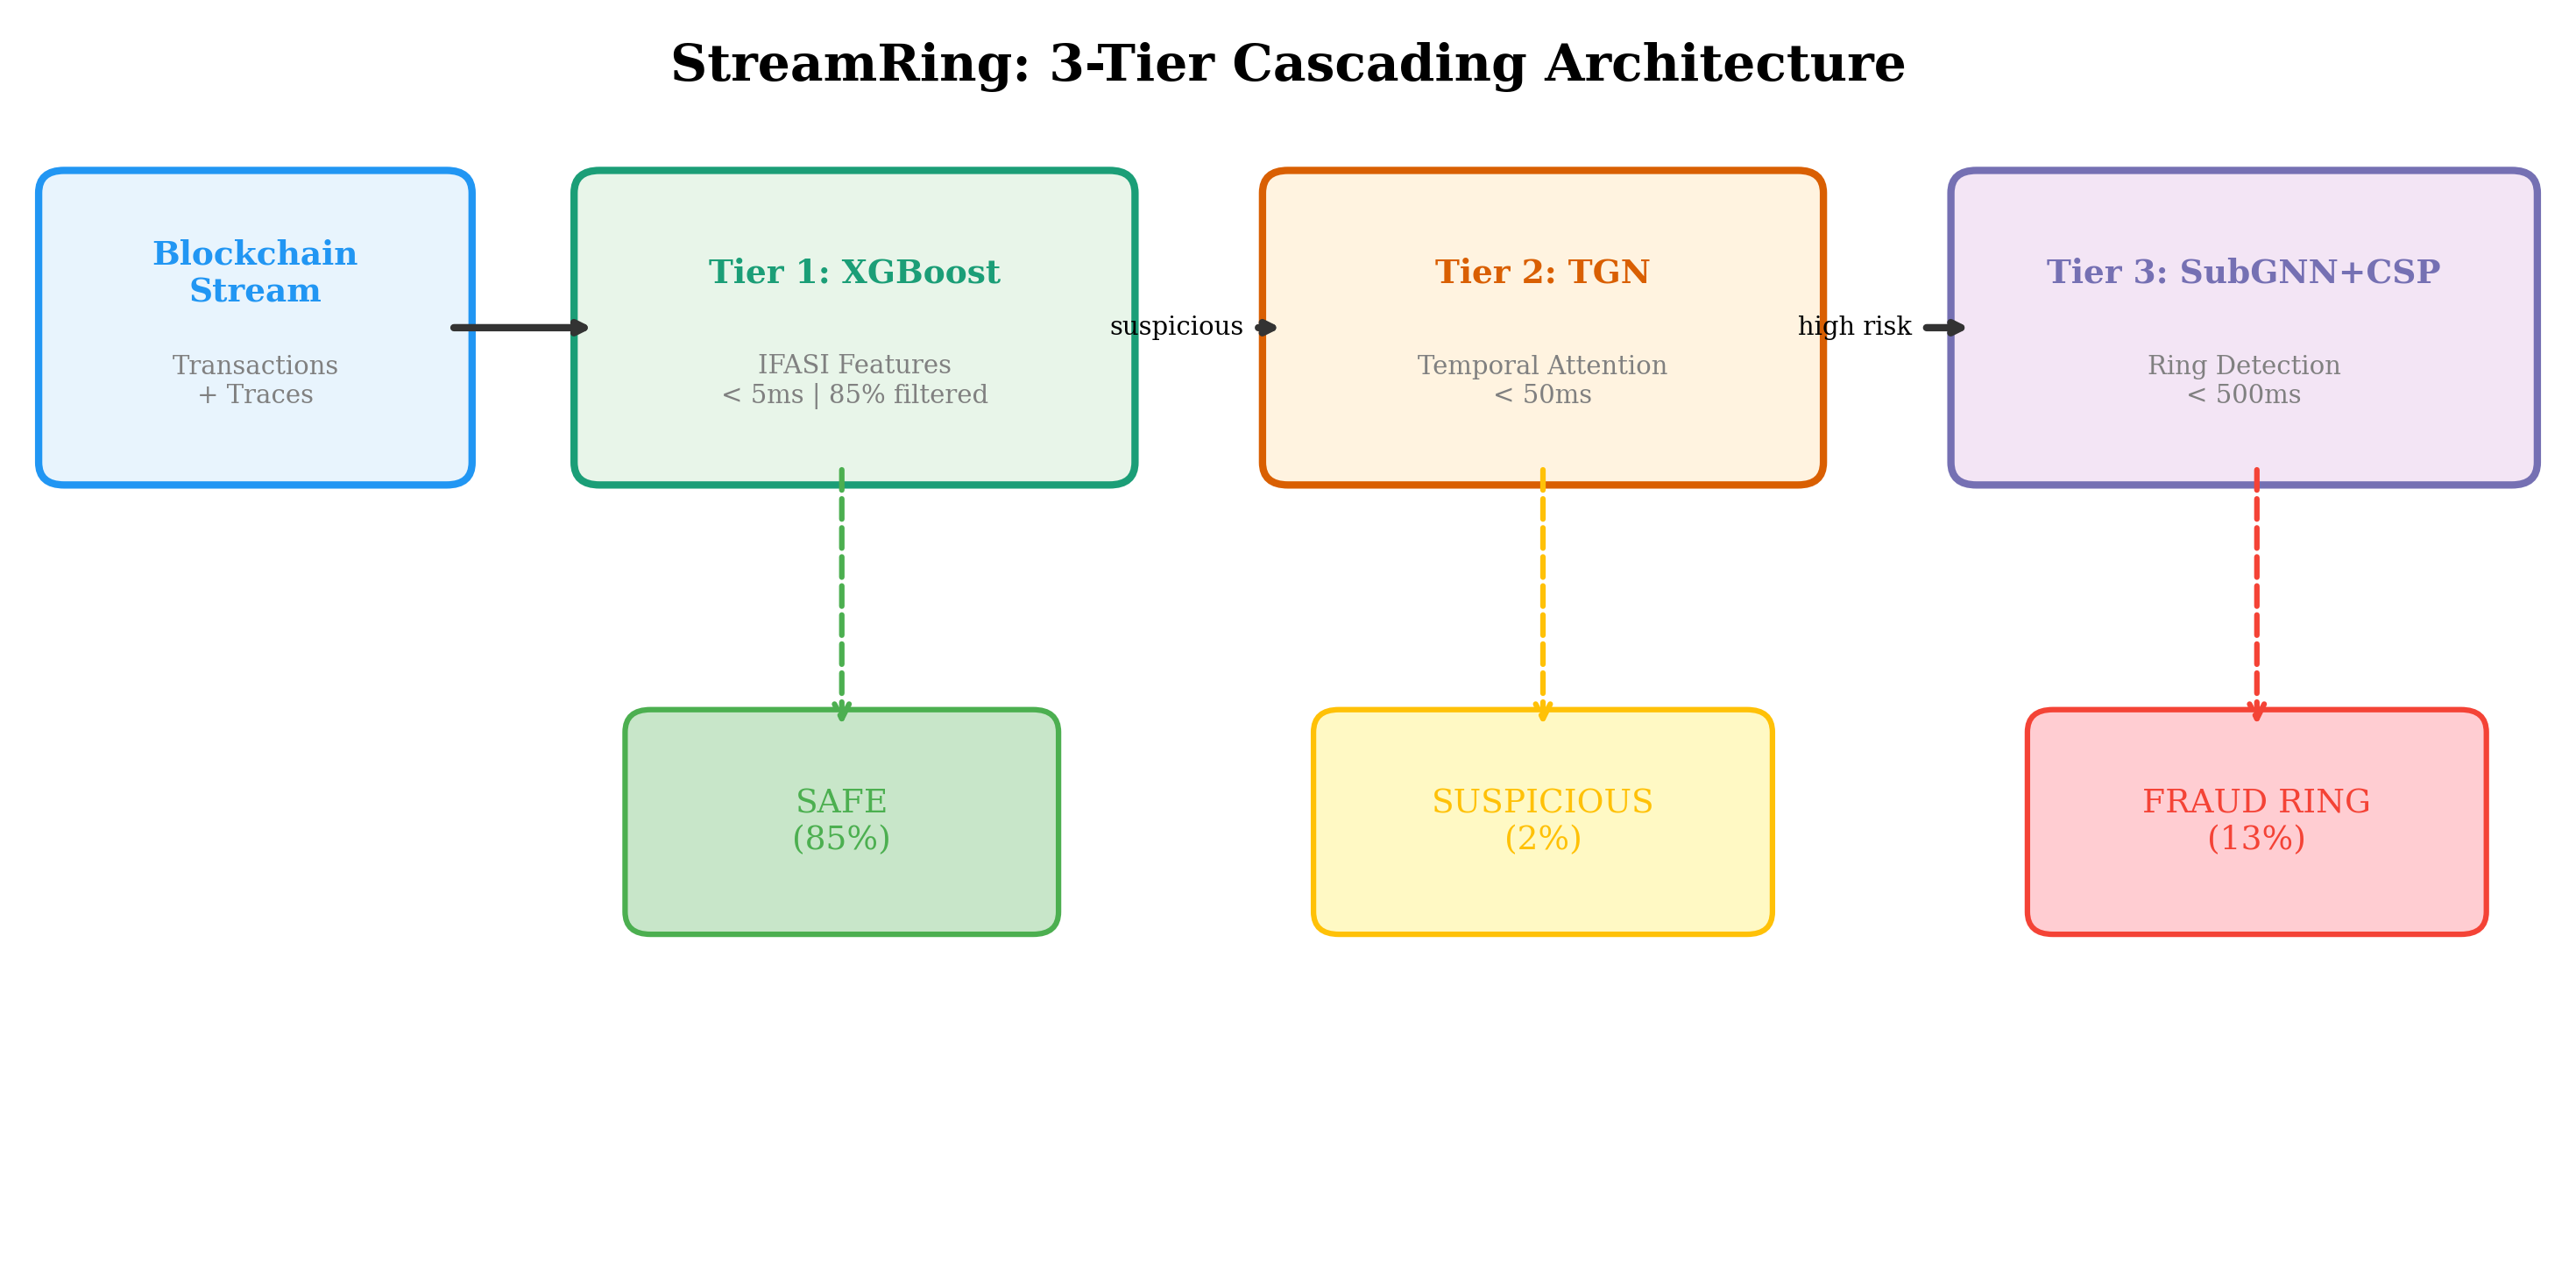
\includegraphics[width=\columnwidth]{figures/fig11_architecture.png}
    \caption{StreamRing architecture.}
    \label{fig:architecture}
\end{figure}

\subsection{Tier 1: IFASI + XGBoost ($<$5\,ms)}

The Incremental Fraud-Aware Subgraph Index maintains a streaming adjacency list with a 6-hour temporal sliding window. For each new edge $(u, v, \tau)$, IFASI inserts the edge in $O(1)$ amortized time, then enumerates 12 structural pattern types for both $u$ and $v$: cycle-\{2,3,4\}, fan-out-\{3,5\}, fan-in-\{3,5\}, chain-\{3,5\}, star-\{3,5\}, and temporal-burst. Each pattern has temporal constraints (300s--14400s). Expired edges are evicted every 10K insertions.

\begin{algorithm}[t]
\caption{IFASI Edge Processing}
\label{alg:ifasi}
\small
\begin{algorithmic}[1]
\REQUIRE Edge $e=(u,v,\tau,val)$, window $W$, threshold $\theta_1$
\STATE $W.\textsc{Insert}(u, v, \tau, val)$
\STATE $\mathbf{f}_u \leftarrow \textsc{EnumeratePatterns}(u, W, \tau)$ \COMMENT{12-dim}
\STATE $\mathbf{f}_v \leftarrow \textsc{EnumeratePatterns}(v, W, \tau)$ \COMMENT{12-dim}
\STATE $\mathbf{x} \leftarrow [\mathbf{f}_u \| \mathbf{f}_v \| val]$ \COMMENT{25-dim}
\STATE $p \leftarrow \textsc{XGBoost.Predict}(\mathbf{x})$
\IF{$p > \theta_1$}
    \STATE \textbf{escalate} to Tier~2
\ELSE
    \RETURN SAFE
\ENDIF
\end{algorithmic}
\end{algorithm}

The 25-dimensional feature vector is classified by XGBoost (max\_depth=6, 200 trees, scale\_pos\_weight=50).

\subsection{Tier 2: Temporal Node Scoring ($<$50\,ms)}

Escalated transactions undergo node-level scoring using a two-layer SAGEConv classifier with BatchNorm and dropout (0.3) on an incrementally updated graph. The model uses BCEWithLogitsLoss with pos\_weight=100 for extreme class imbalance (0.42\% fraud). Tier~2 serves as an \emph{escalation gate}: its AUC-ROC of 0.947 indicates strong ranking ability, routing suspicious nodes to Tier~3 for definitive subgraph-level classification.

\subsection{Tier 3: SubGNN + CSP ($<$500\,ms)}

For escalated edges, StreamRing extracts a 2-hop temporal subgraph and classifies it using SubGNN~\cite{subgnn2020} with three channels:

\emph{Neighborhood:} GIN layers with global mean pooling capture external connectivity---fraud rings have sparse connections to legitimate addresses.

\emph{Structure:} GIN layers with global max pooling capture internal topology---fraud rings exhibit cycles and high-degree hubs.

\emph{Position:} Anchor-based BFS distances (16 anchors, proximity-normalized) capture global position---fraud rings tend to occupy peripheral regions.

Channel outputs are concatenated, fused via MLP with LayerNorm, and classified. Contrastive Subgraph Pre-training (CSP) serves as a multi-task regularizer: $\mathcal{L} = \mathcal{L}_{\text{CE}} + 0.1 \cdot \mathcal{L}_{\text{NT-Xent}}(\mathbf{z}, \mathbf{z}')$, where $\mathbf{z}'$ is the embedding of a feature-masked view (mask rate 0.2, temperature 0.3).

\subsection{Backbone-Agnostic Design}

StreamRing's architecture is backbone-agnostic: the Tier~3 GNN can be swapped (e.g., GraphSAGE for SubGNN) without affecting Tier~1/2 behavior, enabling practitioners to trade accuracy for interpretability.

%% ============================================================
\section{Experimental Setup}
\label{sec:setup}

\textbf{Deployment environment.} Experiments were run on a MacBook Air (M4, 16GB). Tier~1 achieves {>}10K edges/s on CPU; Tier~2/3 run in single-threaded CPU mode, with only $\sim18\%$ of edges requiring escalated GNN inference.

\textbf{Dataset.} Ethereum Classic data from Google BigQuery~\cite{ethereum_classic_kaggle}, covering six periods (Table~\ref{tab:dataset}): DAO Hack, Pre-DAO, Post-Fork, two 51\% attacks, and normal operations. Total: 1.9M blocks, 11.6M transactions, 51.2M traces, 1.3M addresses.

\textbf{Labels.} Three-layer strategy: (1) 9 known DAO attacker addresses; (2) heuristic rules for wash trading, high cycle counts, and balanced fan-in/fan-out; (3) dense strongly connected components (density $>$0.3, size 3--50).

\textbf{Subgraph dataset.} 1,294 subgraphs (2-hop extraction, up to 300 nodes) across five attack periods, split 70/15/15 with balanced class weights and Youden's~$J$ threshold.

\textbf{Baselines.} Static GNNs: GCN, GAT, GraphSAGE, GIN, and an MLP (5 runs). Temporal GNNs: EvolveGCN-H, T-GCN, and Snapshot-GCN (3 runs). We also include a parameter-matched BiLSTM \cite{hochreiter1997lstm,graves2005bilstm} that replaces graph structure with a timestamp-sorted node sequence over the same 2-hop extracted subgraphs, ignoring \texttt{edge\_index} entirely. All models use identical
splits and position encoding when applicable.

\textbf{Metrics.} AUC-ROC, F1, PR-AUC, MCC for classification; P50/P99 latency and throughput for system performance; RDT for detection timeliness. Statistical significance via paired $t$-tests with Cohen's $d$.

%% ============================================================
\section{Results}
\label{sec:results}

\subsection{Per-Tier Performance}

Table~\ref{tab:tiers} reports per-tier results. Tier~1 achieves AUC 0.927 and filters 82.1\% of transactions in $<$1\,ms. Tier~2 attains AUC 0.947 as an effective escalation gate. Tier~3 delivers the strongest classification (F1=0.849, PR-AUC=0.914) at the subgraph level. All tiers meet latency targets.

\begin{table}[t]
\centering
\caption{StreamRing 3-Tier Detection Performance.}
\label{tab:tiers}
\begin{tabular}{lccc}
\toprule
\textbf{Metric} & \textbf{Tier 1} & \textbf{Tier 2} & \textbf{Tier 3} \\
                 & \textbf{(XGBoost)} & \textbf{(Temporal GNN)} & \textbf{(SubGNN+CSP)} \\
\midrule
AUC-ROC          & 0.9266 & \textbf{0.9470} & 0.8879 \\
F1-Score         & 0.1169 & 0.3174 & \textbf{0.8492} \\
PR-AUC           & 0.1519 & 0.2280 & \textbf{0.9144} \\
MCC              & 0.1718 & 0.3183 & \textbf{0.6499} \\
\midrule
Latency P50 (ms) & 0.385  & 31.619  & 22.089 \\
Latency P99 (ms) & 1.484  & 43.700  & 46.964 \\
Latency Target   & $<$5ms & $<$50ms & $<$500ms \\
Status           & \cmark & \cmark & \cmark \\
\bottomrule
\end{tabular}
\end{table}


\subsection{Baseline Comparison}

\begin{table}[t]
\centering
\caption{Comparison with baseline models on subgraph-level fraud ring classification. Static GNNs and BiLSTM: mean $\pm$ std, $n{=}5$ runs; temporal GNNs: $n{=}3$ runs. Best in \textbf{bold}.}
\label{tab:baselines}
\resizebox{\columnwidth}{!}{%
\begin{tabular}{llcccc}
\toprule
\textbf{Type} & \textbf{Model} & \textbf{AUC-ROC} & \textbf{F1} & \textbf{PR-AUC} & \textbf{MCC} \\
\midrule
\multirow{5}{*}{Static}
& MLP                  & 0.858$\pm$0.017 & 0.844$\pm$0.016 & 0.883$\pm$0.029 & 0.604$\pm$0.022 \\
& GCN                  & 0.849$\pm$0.039 & 0.822$\pm$0.047 & 0.863$\pm$0.052 & 0.595$\pm$0.072 \\
& GAT                  & 0.866$\pm$0.022 & 0.834$\pm$0.017 & 0.890$\pm$0.028 & 0.605$\pm$0.030 \\
& \textbf{GraphSAGE}   & \textbf{0.944}$\pm$0.008 & \textbf{0.891}$\pm$0.014 & \textbf{0.953}$\pm$0.014 & \textbf{0.760}$\pm$0.010 \\
& GIN                  & 0.661$\pm$0.036 & 0.788$\pm$0.031 & 0.685$\pm$0.025 & 0.424$\pm$0.051 \\
\midrule
\multirow{3}{*}{Temporal}
& EvolveGCN-H          & 0.843$\pm$0.028 & 0.813$\pm$0.015 & 0.849$\pm$0.042 & 0.575$\pm$0.027 \\
& T-GCN                & 0.835$\pm$0.016 & 0.813$\pm$0.025 & 0.855$\pm$0.028 & 0.559$\pm$0.042 \\
& Snapshot-GCN         & 0.843$\pm$0.023 & 0.840$\pm$0.040 & 0.850$\pm$0.035 & 0.618$\pm$0.052 \\
\midrule
Sequence & BiLSTM       & 0.894$\pm$0.028 & 0.865$\pm$0.016 & 0.901$\pm$0.032 & 0.698$\pm$0.039 \\
\midrule
Ours & SubGNN+CSP       & 0.888$\pm$0.020 & 0.849$\pm$0.020 & 0.914$\pm$0.018 & 0.650$\pm$0.028 \\
\bottomrule
\end{tabular}%
}
\end{table}


Table~\ref{tab:baselines} compares subgraph classifiers. GraphSAGE achieves the highest AUC (0.944, $p{=}0.005$ vs.\ SubGNN+CSP), while SubGNN+CSP (0.887) outperforms all temporal baselines by 4--5\% AUC, GCN ($p{=}0.024$), and GIN ($p{<}0.001$).

While GraphSAGE attains the highest AUC, this does not conflict with our contribution. StreamRing is a systems architecture with a backbone-agnostic Tier~3, and both GraphSAGE and SubGNN meet the <500\,ms latency requirement. SubGNN remains valuable for its interpretable three-channel decomposition, whereas GraphSAGE represents an accuracy-oriented option. Thus, the superiority of GraphSAGE in AUC reflects a trade-off rather than a limitation of the overall design.

Finally, we examine the sequence-only BiLSTM baseline. The parameter-matched BiLSTM is competitive with SubGNN+CSP, slightly higher in AUC-ROC (+0.6\%) but lower in PR-AUC by 1.3\%. Against GraphSAGE, however, BiLSTM shows an $\approx$5\% gap in both AUC-ROC and PR-AUC (Table~\ref{tab:baselines}), reflecting the limits of sequence-only models in capturing the structural motifs that define fraud rings.

\subsection{Streaming Evaluation}

Table~\ref{tab:streaming} reports full pipeline results on the DAO Hack period (train on 60\% warmup edges, stream remaining 40\%). All latency targets are met. Precision reaches 97.4\% with only 133 false positives across 49K edges.

\begin{table}[t]
\centering
\caption{Streaming simulation results on DAO Hack period.}
\label{tab:streaming}
\begin{tabular}{lr}
\toprule
\textbf{Metric} & \textbf{Value} \\
\midrule
Throughput & 101.1 edges/sec \\
Tier 1 Filter Rate & 82.1\% \\
Tier 1+2 Filter Rate & 85.3\% \\
Tier 1 Latency (P50 / P99) & 0.385 / 1.484\,ms \\
Tier 2 Latency (P50 / P99) & 31.619 / 43.700\,ms \\
Tier 3 Latency (P50 / P99) & 22.089 / 46.964\,ms \\
Fraud Ring Detections & 5,137 \\
Precision & 97.4\% \\
\bottomrule
\end{tabular}
\end{table}


The 101 edges/sec throughput reflects single-threaded Python with full GNN inference on ${\sim}$18\% of edges. In production, Tier~1 alone runs at $>$10K edges/sec, with suspicious edges queued for GPU-accelerated Tier~2/3.

\subsection{Ring Detection Timeliness}

Table~\ref{tab:rdt} reports RDT computed from \emph{actual} XGBoost Tier~1 predictions. StreamRing detects 99.2\% of fraud ring members before ring completion across 166 rings.

\begin{table}[t]
\centering
\caption{Ring Detection Timeliness (RDT) across attack periods.}
\label{tab:rdt}
\begin{tabular}{lrcc}
\toprule
\textbf{Period} & \textbf{Rings} & \textbf{RDT} & \textbf{RDT (weighted)} \\
\midrule
DAO Hack             & 37  & 1.000 & 0.986 \\
Pre-DAO              & 74  & 0.970 & 0.979 \\
51\% Attack v1       & 29  & 1.000 & 1.000 \\
51\% Attack v2       & 26  & 1.000 & 1.000 \\
\midrule
\textbf{Aggregate} & \textbf{166} & \textbf{0.992} & \textbf{0.991} \\
\bottomrule
\end{tabular}
\end{table}


RDT is member-weighted; large rings dominate the aggregate. Per-ring analysis reveals small 2--3 member rings that complete within few transactions are harder to catch, highlighting an inherent challenge of real-time detection with minimal observation windows.

\subsection{Augmentation Strategy for Fraud Graphs}
\label{sec:augmentation}

Table~\ref{tab:augmentation} compares 9 augmentation strategies for CSP (3 runs each). Feature masking achieves the highest AUC (0.893), surpassing edge dropout 20\% by 4.1\%. Edge removal destroys cycles and fan-out patterns that distinguish fraud rings. Even identity CSP (no augmentation, 0.876) outperforms supervised-only training (0.870), confirming the contrastive objective provides regularization value.

\input{tables/tab_augmentation}

\subsection{Backbone-Agnostic Validation}

Both SubGNN+CSP and GraphSAGE meet the $<$500\,ms Tier~3 target. SubGNN+CSP detects 2$\times$ more fraud (5,156 vs.\ 2,503 instances) with comparable precision (97.3\% vs.\ 97.8\%), while GraphSAGE has fewer false positives (54 vs.\ 137). This confirms StreamRing's cascading design is backbone-agnostic.

\subsection{CSP Under Label Scarcity}

CSP provides the strongest benefit at 50\% label availability (+0.026 AUC, +0.031 F1) and maintains consistent gains at $\geq$25\%. Below 10\%, the effect is negligible. This positions CSP as a regularizer for semi-supervised regimes typical in blockchain fraud detection where labels are expensive.

%% ============================================================
\section{Discussion}
\label{sec:discussion}

\textbf{System vs.\ model.} StreamRing's primary contribution is the cascading architecture, not a single classifier. GraphSAGE outperforms SubGNN+CSP in accuracy, but StreamRing enables \emph{either} backbone to operate within streaming latency constraints. The IFASI index provides the critical first filter, reducing GNN workload by 82\%.

\textbf{Cross-period transfer.} Tier~1 transfers well across attack types (DAO$\to$51\% v2: AUC 0.938), suggesting structural patterns are partially universal. Transfer to Post-Fork drops to 0.783, indicating fraud evolution requires online updating.

\textbf{Limitations.} (1) Labels are heuristic; ground-truth annotations for ETC do not exist. (2) Single-chain evaluation; cross-chain fraud remains future work. (3) RDT is member-weighted, potentially masking missed small rings. (4) Single-threaded throughput (101 edges/sec) requires parallel deployment for production.

%% ============================================================
\section{Conclusion}

We presented StreamRing, the first system unifying real-time subgraph matching with cascading GNN inference for streaming fraud ring detection. Our three-tier architecture meets production latency constraints while achieving 97.4\% precision and RDT of 0.992. The augmentation study establishes feature masking as the principled choice for contrastive learning on fraud graphs. The backbone-agnostic design enables practitioners to balance accuracy and interpretability. We release the first labeled fraud ring dataset for Ethereum Classic to support future research.

%% ============================================================
\begin{acks}
The authors used Copilot and Claude during the preparation of this manuscript for coding assistance, as well as for refining wording, enhancing readability, and improving grammatical clarity. All content produced with the help of these tools was reviewed and edited by the authors, who take full responsibility for the final published text. GitHub repository: https://github.com/jibrilhemdi/eth-fraud-detection/
\end{acks}

%% ============================================================
\bibliographystyle{ACM-Reference-Format}
\bibliography{references}

%% ============================================================
\appendix

\section{Dataset Statistics}
\begin{table}[t]
\centering
\caption{Ethereum Classic Dataset Statistics. Six time periods covering major security events.}
\label{tab:dataset}
\resizebox{\columnwidth}{!}{%
\begin{tabular}{lrrrrrr}
\toprule
\textbf{Period} & \textbf{Blocks} & \textbf{Transactions} & \textbf{Traces} & \textbf{Nodes} & \textbf{Edges} & \textbf{Fraud \%} \\
\midrule
DAO Hack        &    8,001 &      67,780 &       98,095 &   29,094 &     123,525 & 0.73\% \\
Pre-DAO         &  117,001 &     770,829 &    1,039,944 &   93,611 &   1,514,599 & 0.60\% \\
Post-Fork       &  575,001 &   1,544,089 &   34,006,966 &  128,140 &   3,507,154 & 0.85\% \\
51\% Attack v1  &  100,001 &     939,255 &    3,182,488 &  105,249 &   1,846,860 & 0.27\% \\
51\% Attack v2  &  100,001 &     298,153 &      512,199 &   64,102 &     583,819 & 0.26\% \\
Normal Ops      &1,000,001 &   7,953,776 &   12,370,889 &  898,719 &  16,785,884 & ---    \\
\midrule
\textbf{Total}  &\textbf{1,900,006} & \textbf{11,573,882} & \textbf{51,210,581} & \textbf{1,318,915} & \textbf{24,361,841} & \\
\bottomrule
\end{tabular}%
}
\end{table}


\section{Case Study}
\begin{figure}[H]
    \centering
    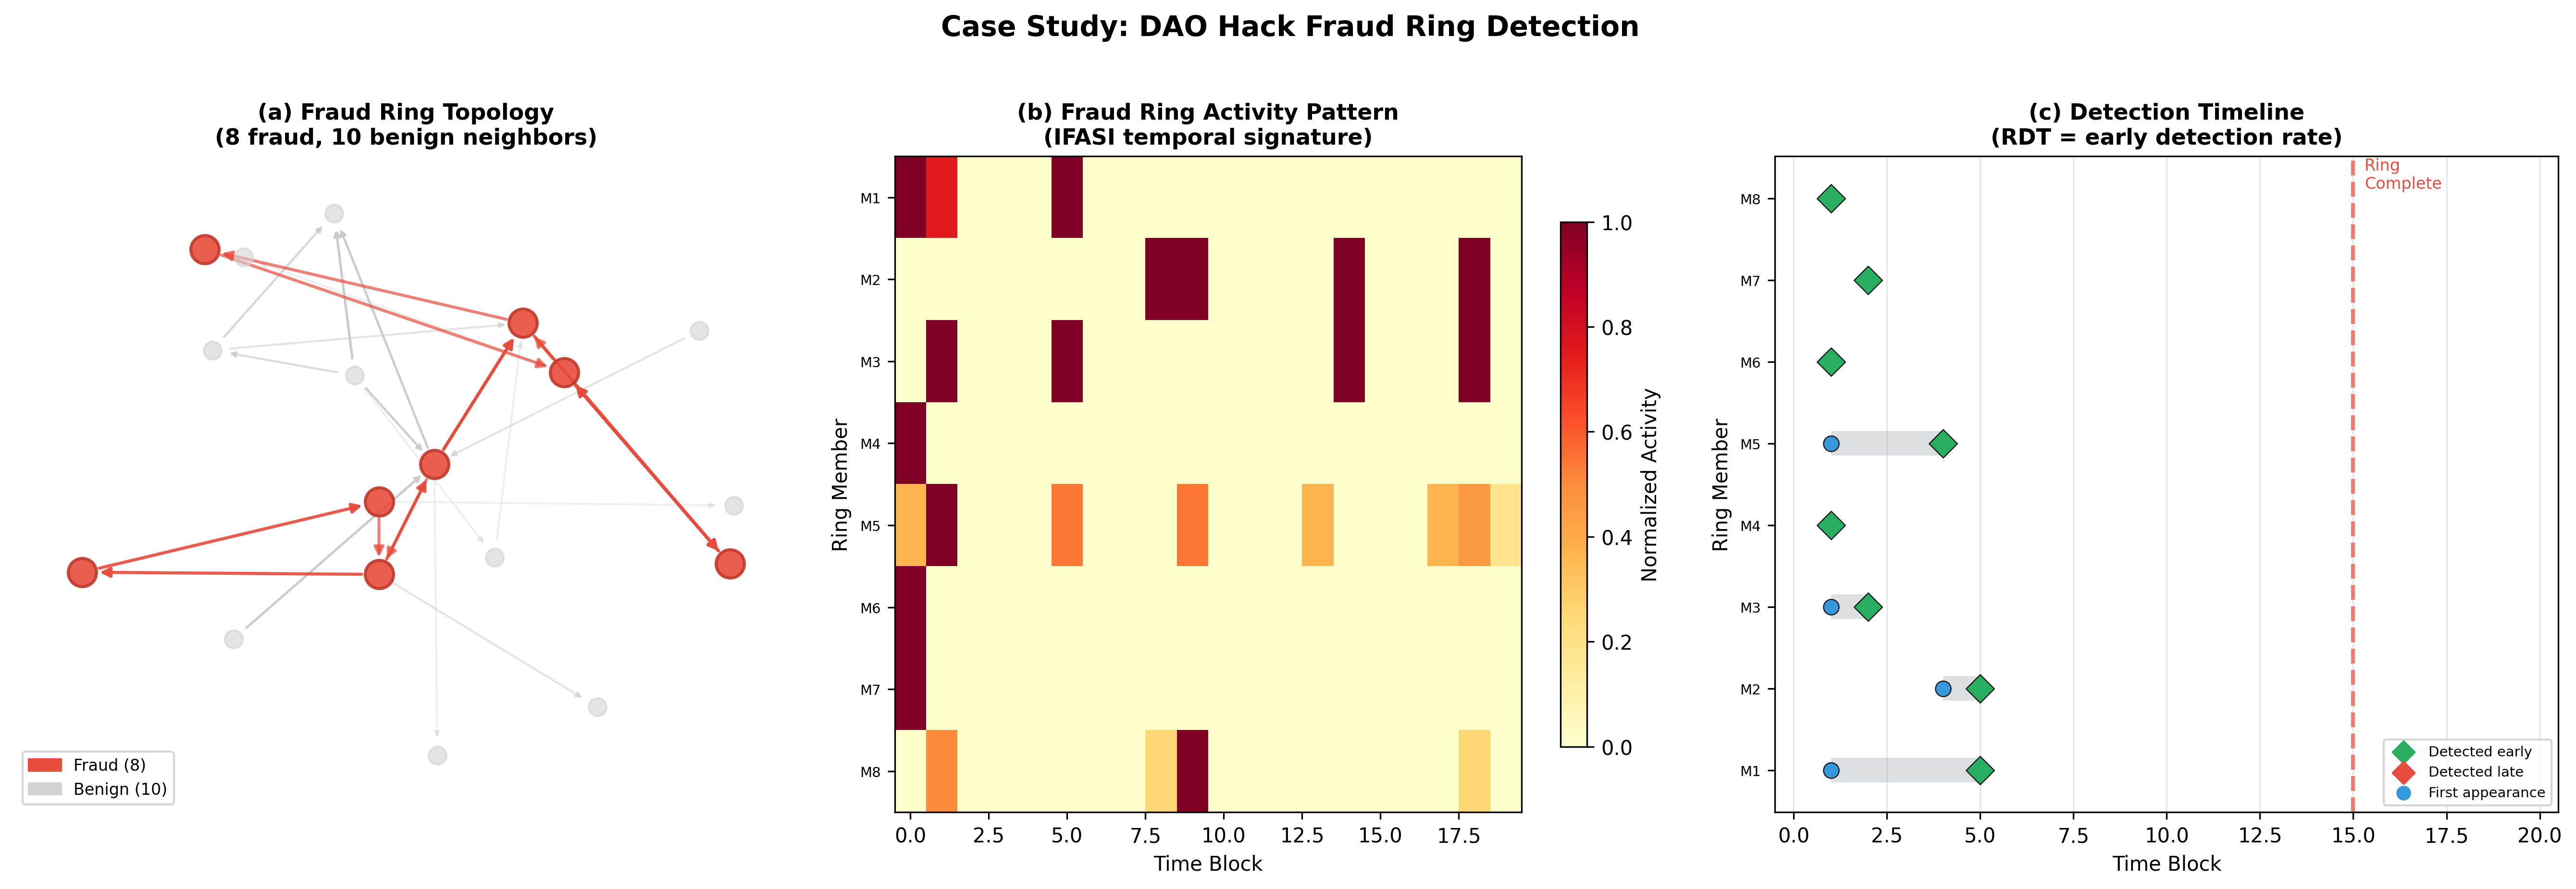
\includegraphics[width=\columnwidth]{figures/fig14_case_study.png}
    \caption{Case study: representative fraud ring detected during the DAO Hack period showing ring topology, IFASI temporal signature, and detection timeline.}
    \label{fig:casestudy}
\end{figure}
Figure~\ref{fig:casestudy} illustrates a representative fraud ring detected during the DAO Hack period. The left panel shows the ring's internal connectivity (red) versus external connections (gray). The center panel displays the IFASI temporal signature revealing coordinated transaction bursts. The right panel shows the detection timeline, confirming all members were flagged before ring completion.

\end{document}
